In this section, describe \emph{what you did}. Roughly speaking, explain what data you worked with, how or from where it was collected, it's structure and size. Explain your analysis, and any specific choices you made in it. Depending on the nature of your project, you may focus more or less on certain aspects. If you collected data yourself, explain the collection process in detail. If you downloaded data from the net, show an exploratory analysis that builds intuition for the data, and shows that you know the data well. If you are doing a custom analysis, explain how it works and why it is the right choice. If you are using a standard tool, it may still help to briefly outline it. Cite relevant works. You can use the \verb|\citep| (whole citation in parenthesis) and \verb|\citet| (only year in parenthesis) commands for this purpose \citep{mackay2003information}.

% This is the template for a figure from the original ICML submission pack. In lecture 10 we will discuss plotting in detail.
% Refer to this lecture on how to include figures in this text.
% 
% \begin{figure}[ht]
% \vskip 0.2in
% \begin{center}
% \centerline{\includegraphics[width=\columnwidth]{icml_numpapers}}
% \caption{Historical locations and number of accepted papers for International
% Machine Learning Conferences (ICML 1993 -- ICML 2008) and International
% Workshops on Machine Learning (ML 1988 -- ML 1992). At the time this figure was
% produced, the number of accepted papers for ICML 2008 was unknown and instead
% estimated.}
% \label{icml-historical}
% \end{center}
% \vskip -0.2in
% \end{figure}

\subsection{Data}
Obtaining non-sparse data for all countries in the world over a long time horizon is quite challenging.

We began by exploring ourselves if cardiovascular diseases are in Germany truly abnormal with comparison to the rest of the world. In all of our analysis we wanted to include a closer comparison with high-income countries since Germany is one of them and comparing countries with similar healthcare and gdp could lead to more concrete results. There is not a wide variety of enormous datasets including data about all countries over a long time period and the one that we decided to use for Figure \ref{Cardiovascular diseases over time} was the Global Burden of Disease study \citep{GBD2019}. The filtering on their website makes it easy to download only the data we truly needed. We obtained information about the death rate and incidence rate of CVDs for all countries divided into 5-year age groups for years 1990-2019. The data also included a lower and upper bound for uncertainty. The only change we did outselves was leaving only the rows corresponging to the sum of all age groups.

Furthermore, CVDs are a group of diseases and to get to the root of the issue we needed to investigate which specific diseases from this group take up the majority of cases. For this we went back to \citep{GBD2019} and requested data about specific CVDs. There was too much data for one file which meant that we had to combine files and filter out unwanted data as to leave us only with the number of deaths grouped by disease only for Germany. 
% THIS IS STILL IN THE OLD REPO 

Since a disease death rate and incidence rate may largely rely on the healthcare system of a country. Thus, we used healthcare expenditure as the percentage of GDP from \citep{health_expenditure} as to indicate whether a country has a high quality medical system.

When it comes to causes, CVDs are likely influenced by a range of factors. These include dietary habits, especially fat consumption as detailed in \citep{fat_consumption}, where the data is measured in daily fat intake per person. Lifestyle choices such as alcohol consumption, referenced from \citep{alcohol_consumption}, are quantified by annual sales of pure alcohol in liters per person aged 15 and older. The role of smoking in CVDs prevalence is also considered, with data sourced from \citep{smoking}, highlighting the percentage of the population over 15 years old who smoke daily. Additionally, the impact of an aging population on CVDs is a significant factor, as indicated by demographic data from \citep{age}, suggesting potential correlations. 

A key challenge on using data from various sources lies in consistency. They might differ in the number of countries, years of study, and some even contains missing data for different years. See table 1 for details. As a result, we ended up choosing a mutual set of 178 countries and a date range from 1990 to 2019 to perform analysis on, which balance between data quantity and the number of missing values. The joining process is done using the ISO-3 country code.


\begin{tabular}{|p{2cm}|p{1cm}|p{2cm}|p{2cm}|}
\hline
Data source & Number of countries & Year range & Percentage of missing data from 1990 - 2021\\
\hline
Global Burden Disease IHC & 206 & 1990 - 2019 & 0\%\\
Health expenditure & 266 & 1960 - 2022 & 41\%\\
Fat consumption & 194 & 1961 - 2020 & 0\%\\
Alcohol consumption & 187 & 2000 - 2019 & 0\%\\
Population age & 238 & 1950 - 2100 & 0\%\\
\hline
\end{tabular}
Table 1


\begin{figure*}[h]
    \vskip 0.2in
    \centering
    \centerline{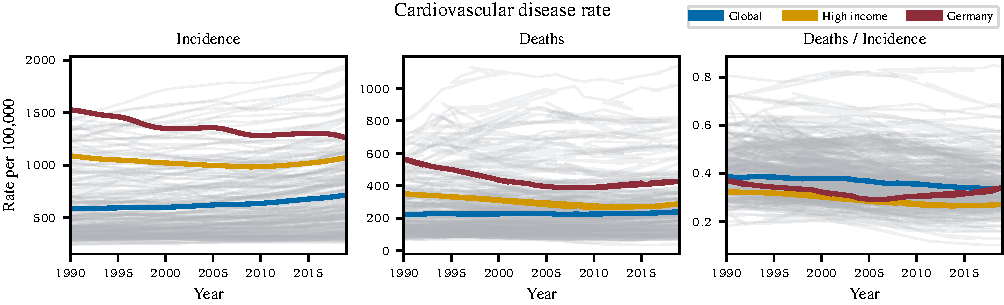
\includegraphics[]{fig/fig_cardiovascular_disease_rate.pdf}}
    \caption{Effect of the cardiovascular diseases on the world over time. From left to right: incidence rate, death rate, 
    and the ratio of death rate to incidence rate. The data is taken from the Global Burden of Disease study \citep{GBD2019}. We specifically focus on the values 
    for Germany in comparison to other high income countries and the world.}
    \label{Cardiovascular diseases over time}
\end{figure*}